\section{Waiting Time}
\label{sec:waitingTime}

The waiting time function is used to calculate the total time advertisers have to wait before being admitted to the ad cache. 
The function directly shapes the structure of the ad cache,  determines its diversity and performs flow control. 
It also protects against attacks, where a malicious actor tries to dominate the ad cache and exhaust resources of the registrar. 

Each request is given a waiting time based on the IP address of the registrar, the topic of the request and the current state of the ad cache. 
The waiting time function is divided into three parts: \emph{occupancy score} (ranging from $0$ to $\infty$) and  \emph{similarity score} (ranging from $0$ to $2$) and is normalized by the amount of time each ad spent in the cache $a$ (\ie \emph{ad lifetime}). $a$ determines the absolute values of the returned waiting time. The final result is a product of all three: $w = a \times \textit{occupancy score} \times \textit{similarity score}.$

The \emph{occupancy score} is based uniquely on the number of the ads already in the cache.
Its role is to progressively increase the waiting time as the ad cache fills up and to limit the memory used by a registrar.
The \emph{occupancy score} is defined by equation~\ref{eq:occupancy}:

\begin{equation}
\label{eq:occupancy}
    \textit{occupancy score} = \frac{1}{(1-\frac{d}{n})^{P_{occupancy}}}
\end{equation}
where $d$ is the number of ads in the cache, $n$ is the capacity of the cache, and $P_\textit{occ}$ is a protocol parameter. 
When the number of ads in the cache is low ($d \ll n$ ), the \emph{occupancy score} goes to $1$. 
As the ad cache fills up, the score will be amplified by the divisor of the equation. 
The higher values of $P_\textit{occ}$, the faster the increase. 
With the current occupancy $d$ close to the capacity of the cache $n$, the \emph{occupancy score} goes to infinity thus limiting the number of admitted requests. We analyse the behavior of the waiting function and choose optimal system parameter values in \Cref{sec:analysis}.

The role of the \emph{similarity score} is to determine how similar is the incoming request to the ads already in the ad cache in terms of the IP address and the topic. 
Requests significantly different from the current content of the cache receive lower similarity score resulting in lower overall waiting time. 
Such an approach promotes fairness across topics (it is easier for less popular topics to get into the cache) and protects against attempts to fill the ad cache by a small number of advertisers (as identified by their IP addresses). The similarity score is defined as a sum of similarity score for IP and the topic of the request and a system parameter $b$: $\textit{similarity} = b + \textit{similarity(topic)} + \textit{similarity(IP)}$. 

The system parameter $b$ ensures that the waiting time never reaches $0$ even when requests get $0$ values for IP and topic similarity score. Together with $P_\textit{occ}$, it shapes the behaviour of the waiting functions. We choose values for those parameters in \Cref{sec:analysis}.

The similarity score for topics is given by equation~\ref{eq:similarity}:
\begin{equation}
\label{eq:similarity}
    \textit{similarity(topic)}= \frac{d(topic)}{d}
\end{equation}
where $d(topic)$ is the number of ads for the specified topic already in the cache and $d$ is the total number of ads in the cache. 
The score goes to $1$ as the specified topic dominates the cache $d(topic)  \approx  d$. 

%For calculating the IP address diversity \sysname uses a different similarity score. 
A simple similarity score used for topics cannot be securely applied for IP addresses. 
An attacker may be able to generate a large number of different addresses sharing the same prefix (\eg using a single /24 IPv4 network) that, while similar, would receive low \emph{similarity scores}. 
A common solution (\eg adopted by the Go Ethereum client~\cite{geth}) limits the number of IP addresses coming from the same (\eg /24 IPv4 address) network.
However, it is impossible to reliably set those limits without knowledge about the network size or NAT configuration of the honest nodes. 
Instead, we propose an approach that directly captures the similarity level across different IPs and translates it into a numerical score. 

We introduce a binary \emph{tree}, as shown on \Cref{fig:ip_tree}, that stores IP addresses used in the existing registrations in the ad cache.
Each node stores a counter, while the edges represent consecutive $0$s or $1$s in a binary representation of IP addresses.
For simplicity,  we present the \emph{tree} for IPv4 addresses but its adaptation for IPv6 is straightforward.

\begin{figure}
    \includegraphics[width=0.45\textwidth]{img/ip_tree}
    \caption{Inserting an IP address into the IP \emph{tree} structure. \mk{TODO:make it up to date, smaller and consistent with other figures.}}
    \label{fig:ip_tree}
\end{figure}

Apart from its root,  the \emph{tree} consists of 32 levels (33 levels in total) representing bits in the binary representation of IPv4 IP addresses. 
The root level is depicted as level $0$, the level of its successor as level $1$ and so on. 
The counter of every \emph{tree} node is initially set to $0$. When adding an IP to the \emph{tree},  the address is first converted to its binary representation and follows a path in the \emph{tree} corresponding to consecutive bits. 
Counters of all the visited nodes are increased by $1$. 
As a result, the root counter stores the number of all the IP addresses in the ad cache, its $0$ successor stores the number of the IP addresses starting with $0$, its $1$ successor stores the number of the IP addresses starting with $1$ and so on. 
Removing an IP from the \emph{tree} follows the analogical procedure but decreases all the counters on the path. 

After each addition of an address to the \emph{tree} a score is generated.
The score is a sum of \emph{penalty points} of obtained on visited nodes. 
$$score(IP)=\sum_{i=1}^{32} \textit{penalty}(p_{\geq i}) $$
where $p_{\geq i}$ is the number of IP addresses in the cache sharing a prefix with $IP$ with a length of at least $i$. A penalty point is given at $p_{\geq i}$ if the IP address to be added makes the tree more unbalanced than the tree currently is:

\begin{equation}
    \textit{penalty}(p_{\geq i})=
    \begin{cases}
      0, & \text{if}\ p_{\geq i} \leq \frac{p_0}{2^i} \\
      1, & \text{otherwise}
    \end{cases}
  \end{equation}

The counter values are taken \emph{before} the increment caused by adding the address\footnote{The first added address will thus always have a score of $0$}. 
Finally, the similarity score for an IP is normalized by the length of the IP address (and thus the maximum possible number of the penalty points):
\begin{equation}
    \textit{similarity(IP}) = \frac{\textit{score(IP)}}{32}
\end{equation}

Similarly to the topic score, the IP similarity score ranges from $0$ to $1$ and returns values closer to 1 for different addresses sharing the same prefix (the longer the shared prefix, the higher the score).

The final formula for the waiting time function can be represented with  the following formula:%,  adding all \emph{similarity scores} and multiplying by the \emph{occupancy score}:

\begin{equation}
\begin{split}
    \textit{w(IP, topic)} = 
    a(b + \frac{d(topic)}{d} + \frac{\textit{score(IP)}}{32}
    )
    \frac{1}{(1-\frac{d}{n})^{P_\textit{occ}}}
\end{split}
\end{equation}

%The formula can be simplified like in equation~\ref{eq:simp}, where ss determines the the \emph{similarity score} and os the \emph{occupancy score}.

%\begin{equation}
%\label{eq:simp}
%    \textit{w(IP, topic)} = 
%    (\textit{ss(IP)} + 
%    \textit{ss(topic)})
%    \textit{os()}
%\end{equation}

\subsection{Lower Bound}
With the waiting time formula, every change in the registrations stored in  the ad cache may increase or decrease waiting times of other requests. 
Therefore, an advertiser receiving waiting time $w(t_1)$ at time $t_1$, may get a smaller waiting time $w(t_2)$ at time $t_2$ ($t_1 < t_2$) in case the content of the ad cache is different (\eg when an ad for the same topic expires between $t_1$ and $t_2$). 
As a result, advertisers are incentivized to keep checking the waiting times as frequently as possible hoping for a better one and generating unnecessary overhead in the system.
%Registration ticket requests should be kept to the minimum and an incentive for constantly spamming ticket requests to get a better waiting time can overload a network and can lead to some nodes getting better performance than the rest.
To prevent this behaviour, we design a mechanism ensuring that any node already in possession of a ticket with a determined waiting time, cannot get a better waiting time (including the new waiting time and the time passed between the first ticket request and the subsequent) by sending new ticket requests.
One solution to this problem is to take into account all the expiration times when calculating the waiting time. 
However, it is computationally expensive (\eg $O(d)$ per request) and unfeasible in practice as it open a Denial of Service vector of attack.

\begin{figure}
    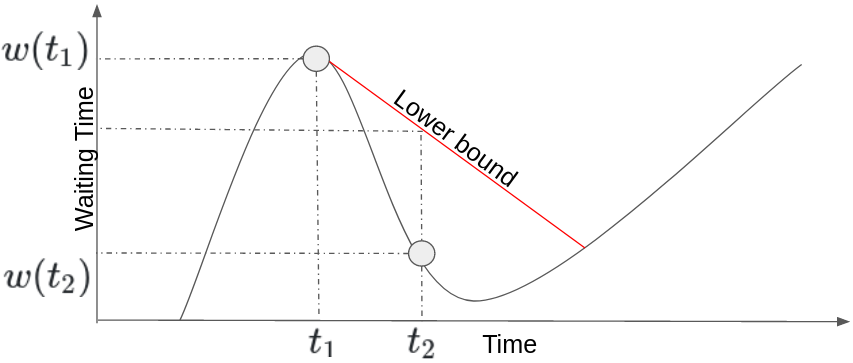
\includegraphics[width=0.45\textwidth]{img/lower_bound.png}
    \caption{Waiting time lower bound.}
    \label{fig:lower_bound}
\end{figure}

When asking for a new waiting time before the previously obtained one elapses,
an advertiser loses its already accumulated waiting time. This means that
asking for a new waiting at time $t_2$ can lower the overall waiting only if
the new waiting time $w(t_2)$ is smaller than $w(t_1)$ by more than the time elapsed $t_2 - t_1$: $w(t_1) - w(t_2) < t_2 - t_1$.
To make sure this is not the case, our protocol enforces a lower bound on the
waiting time. \Ie we make sure that an advertiser's waiting time received at
$t_2$ is not smaller than the waiting time at $t_1$ ($t_1 < t_2$) by more than
$t_2 - t_1$ (\Cref{fig:lower_bound}).
However, holding such a bound for every request (\ie every combination of IP/topic) would cause significant memory overhead ($O(|IPs|\times|topics|)  \gg O(d)$) and would present an easy way for an attacker to create additional state at the registrar. 

To store the lower bound in a more efficient way, we rewrite the waiting formula as a sum:
\begin{equation}
\begin{split}
    \textit{w(IP, topic)} = 
    \frac{ab}{(1-\frac{d}{n})^{P_\textit{occ}}} + \frac{ad(topic)}{d(1-\frac{d}{n})^{P_\textit{occ}}} + \frac{\textit{score(IP)}}{32(1-\frac{d}{n})^{P_\textit{occ}}}
\end{split}
\end{equation}


Ensuring that the lower bound is enforced for each of the three components
makes sure that the total waiting will respect the lower bound as well. At the
same time, it only requires storing the lower bound for every IP/topic in the table and not all their combinations. This approach reduces the memory overhead to $O(|IPs|+|topics|) = O(d)$.

\sysname keeps a lower bound for each IP and topic in the ad cache. When a specific topic enters the cache for the first time, bound(topic) is set to 0 and a timestamp(topic) is set to the current time. When a ticket request arrives for the same topic, we calculate the IP waiting time $w_{\textit{topic}}$ and return the value, $w_{\textit{topic}} = \textit{max}(w_{\textit{topic}}, \textit{bound}(\textit{topic}) - \textit{timestamp}(\textit{topic}))$. The bound and the timestamp are updated when a new ticket is issued and $w_{\textit{topic}} > (\textit{bound}(\textit{topic}) - \textit{timestamp}(\textit{topic}))$. 

\hl{The same holds for topics.}
\mk{TODO: @Onur we need to introduce the waiting time in the tree I believe}


